\documentclass[hyperref={pdftex,unicode}]{beamer}

%%% Поля и разметка страницы %%%
\usepackage{pdflscape}   % Для включения альбомных страниц
\usepackage{geometry} % Для последующего задания полей
\usepackage{setspace} % Для интерлиньяжа
\usepackage[14pt]{extsizes}
\usepackage{titlesec}
\usepackage{tocloft}
\usepackage{enumitem}
\usepackage{fancyhdr}

%%% Кодировки и шрифты %%%
\usepackage{cmap}                    % Улучшенный поиск русских слов в полученном pdf-файле
\usepackage[T2A]{fontenc}	     % Поддержка русских букв
\usepackage[utf8]{inputenc}	     % Кодировка utf8
\usepackage[english=nohyphenation,russian=nohyphenation]{hyphsubst} % Запрет переносов
\usepackage[english, russian]{babel} % Языки: русский, английский
% \usepackage{pscyr}						% Красивые русские шрифты

%%% Математические пакеты %%%
\usepackage{amsthm,amsfonts,amsmath,amssymb,amscd} % Математические дополнения от AMS

%%% Оформление абзацев %%%
\usepackage{indentfirst} % Красная строка

%%% Цвета %%%
\usepackage[usenames]{color}
\usepackage{color}
\usepackage{colortbl}

%%% Таблицы %%%
\usepackage{longtable}		     % Длинные таблицы
\usepackage{multirow,makecell,array} % Улучшенное форматирование таблиц

%%% Общее форматирование
\usepackage{caption}
\captionsetup[figure]{labelsep=space,justification=centering,singlelinecheck=false}

\usepackage{soul}                    % Поддержка переносоустойчивых подчёркиваний и зачёркиваний
\usepackage{multicol}

%%% Библиография %%%
\usepackage{cite} % Красивые ссылки на литературу

%%% Гиперссылки %%%
\usepackage[unicode,plainpages=false,pdfpagelabels=false]{hyperref}

%%% Изображения %%%
\usepackage{graphicx} % Подключаем пакет работы с графикой
../../../../template/lab/sys/styles.tex

\definecolor{primary}{HTML}{0D47A1}
\definecolor{accent}{HTML}{AFB42B}
\setbeamercolor*{palette primary}{fg=white,bg=primary}
\setbeamercolor*{enumerate item}{fg=accent}
\setbeamercolor*{itemize item}{fg=accent}

\title{Программный модуль учета персональной финансовой информации}
\author{%
  Будный Р. И., студент гр. 120602 \\
  Сальников А. А., ведущий инженер-программист \\
  Лаппо А. И., ассистент кафедры ИТАС
}
\date{2016}

\begin{document}

\begin{frame}
  \maketitle
\end{frame}

\begin{frame}{Введение}
  Предмет работы: мобильное приложение.

  \smallskip
  Назначение: учет персональной финансовой информации.

  \smallskip
  Обоснование:
  \begin{itemize}
  \item популярность темы разработки мобильных приложений;
  \item необходимость учета баланса личных финансов;
  \item желание изучить тему компьютерного зрения.
  \end{itemize}
\end{frame}

\begin{frame}{Аналоги}
  7 аналогов, 3 группы:
  \begin{enumerate}
    \item платные, много функций (4);
    \item бесплатные, много функций (1);
    \item бесплатные, мало функций (2).
  \end{enumerate}
\end{frame}

\begin{frame}{Постановка задачи}
  Системные требования:
  \begin{itemize}
    \item ОС Android 4.0;
    \item не требует доступа к сети Интернет и личным данным;
    \item открытое и бесплатное.
  \end{itemize}

  \smallskip
  Минимальный набор функций:
  \begin{itemize}
  \item ведение нескольких счетов учета;
  \item поддержка нескольких валют учета;
  \item редактирование категорий учета.
  \end{itemize}
\end{frame}

\begin{frame}{Структура}
  \begin{figure}[h!]
    \centering
    \includegraphics[width=\textwidth]{fig/design_main.eps}
  \end{figure}
\end{frame}

\begin{frame}{Информационное обеспечение}
  Ввод данных:
  \begin{itemize}
    \item ручной;
    \item автоматический.
  \end{itemize}

  \smallskip
  Вывод данных:
  \begin{itemize}
    \item хронологический порядок;
    \item группировка по категориям учета.
  \end{itemize}
\end{frame}

\begin{frame}{Алгоритмическое обеспечение}
  \begin{minipage}{0.6\linewidth}
  Автоматический механизм ввода:
  \begin{itemize}
    \item распознавание числовых данных по изображению с фотокамеры;
    \item метод опорных векторов, гистограммы ориентированных градиентов;
    \item обучение модели классификатора на ПК разработчика.
  \end{itemize}
  \end{minipage}
  \hfill
  \begin{minipage}{0.35\linewidth}
    \begin{figure}[h!]
      \centering
      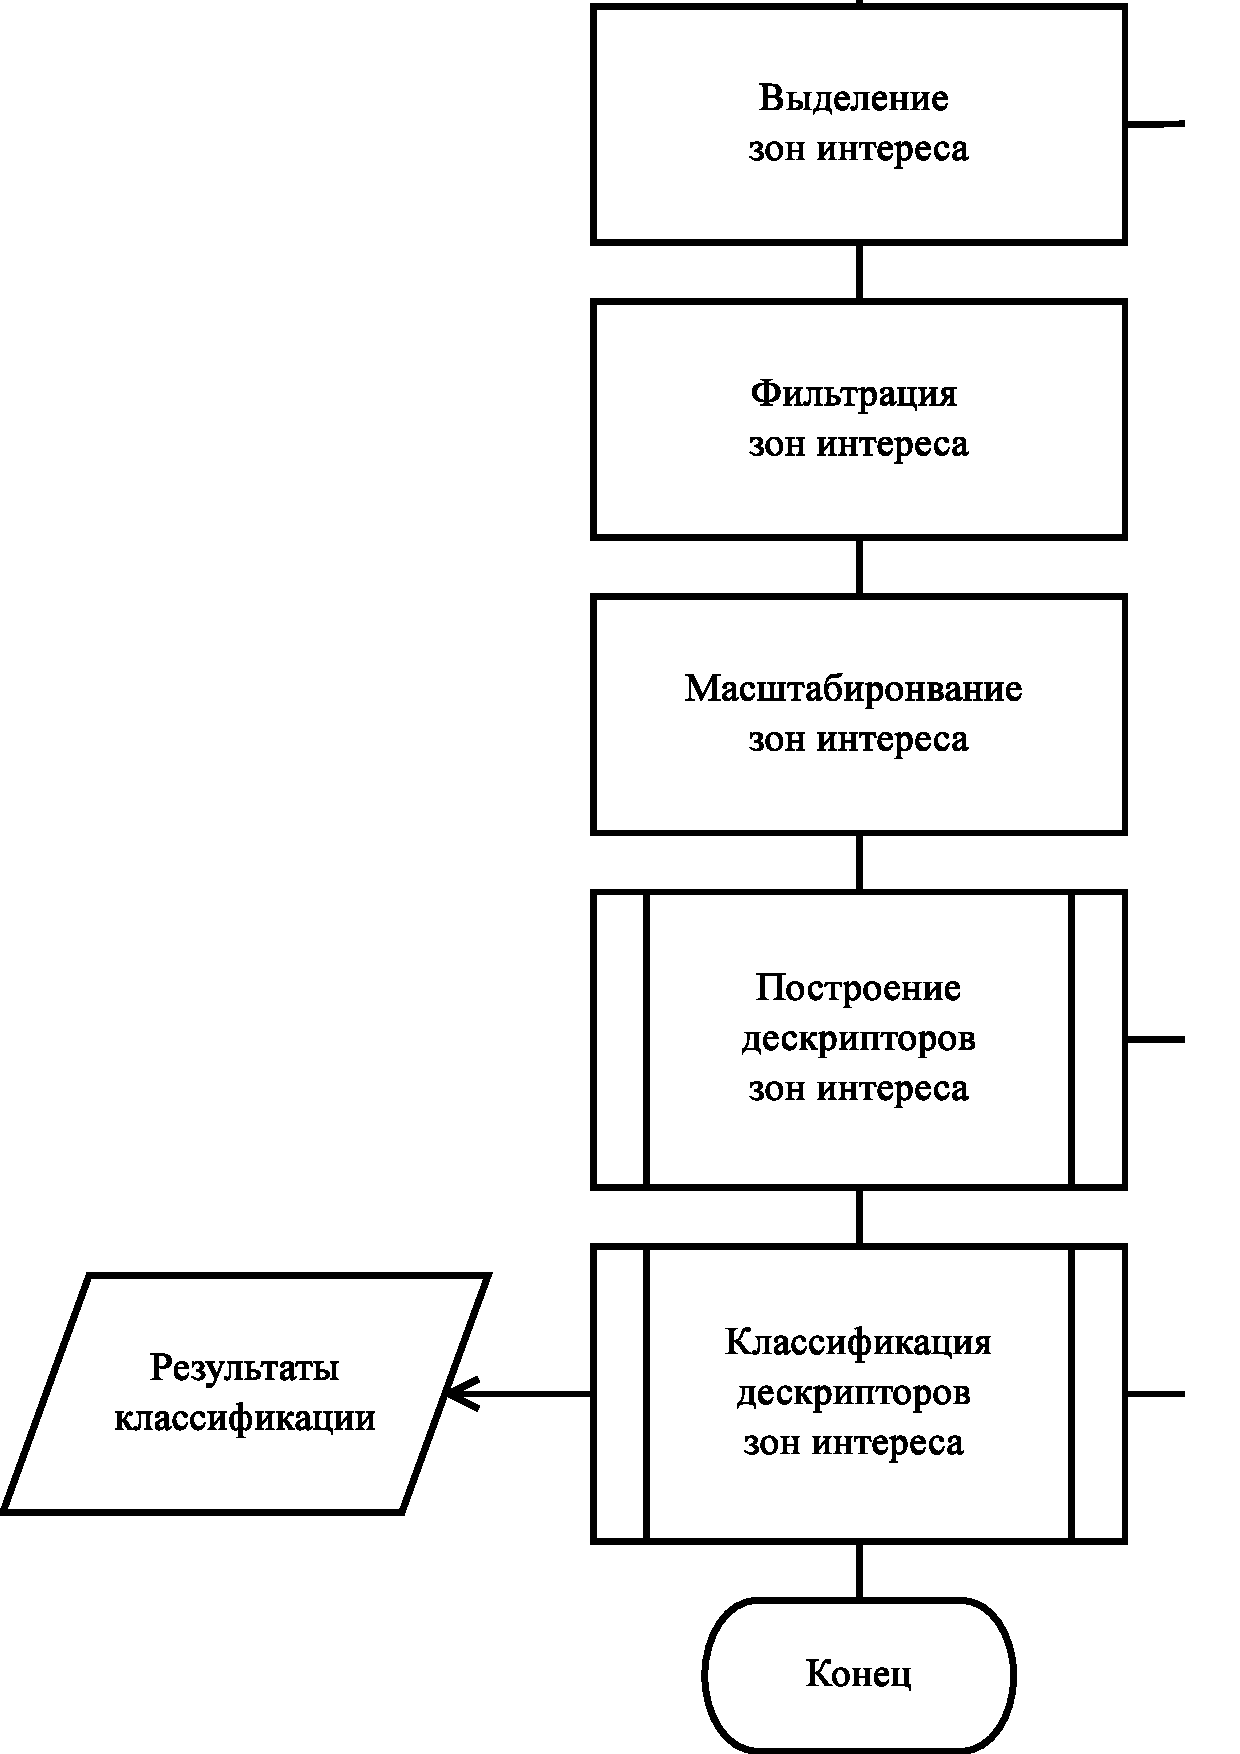
\includegraphics[width=\textwidth]{fig/implementation_cv_recognition.png}
    \end{figure}
  \end{minipage}
\end{frame}

\begin{frame}{Пользовательский интерфейс}
  \begin{minipage}{0.55\linewidth}
    Основные цели:
    \begin{itemize}
    \item удобство использования;
    \item минимум действий при вводе;
    \item соответствие Material Design.
    \end{itemize}

    Результат:
    \begin{itemize}
    \item макеты экранов;
    \item схема переходов.
    \end{itemize}
  \end{minipage}
  \hfill
  \begin{minipage}{0.35\linewidth}
    \begin{figure}[h!]
      \centering
      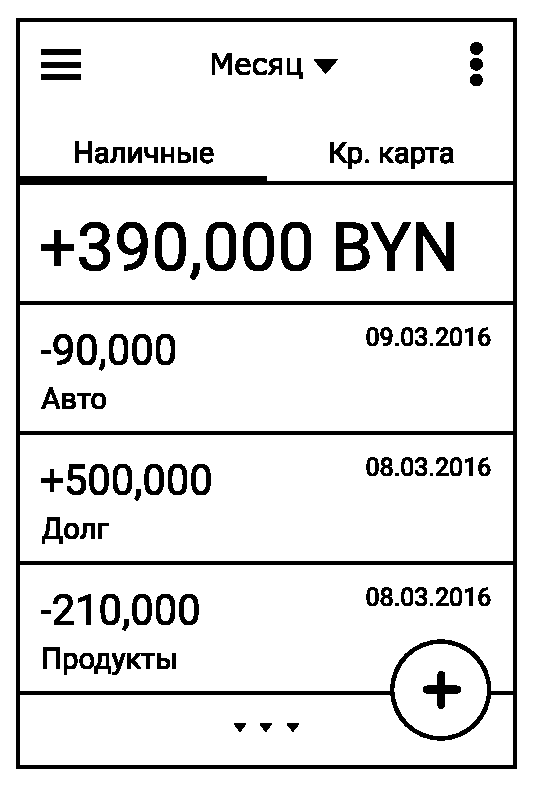
\includegraphics[width=\textwidth]{fig/ui_activities_balance_text_chrono.eps}
    \end{figure}
  \end{minipage}
\end{frame}

\begin{frame}{Детали реализации}
  \begin{itemize}
    \item языки программирования: Java, C++;
    \item СУБД Realm;
    \item \texttt{long} для хранения величин транзакций;
    \item распознавание изображений: OpenCV.
  \end{itemize}
\end{frame}

\begin{frame}{Руководство пользователя}
  \centering
  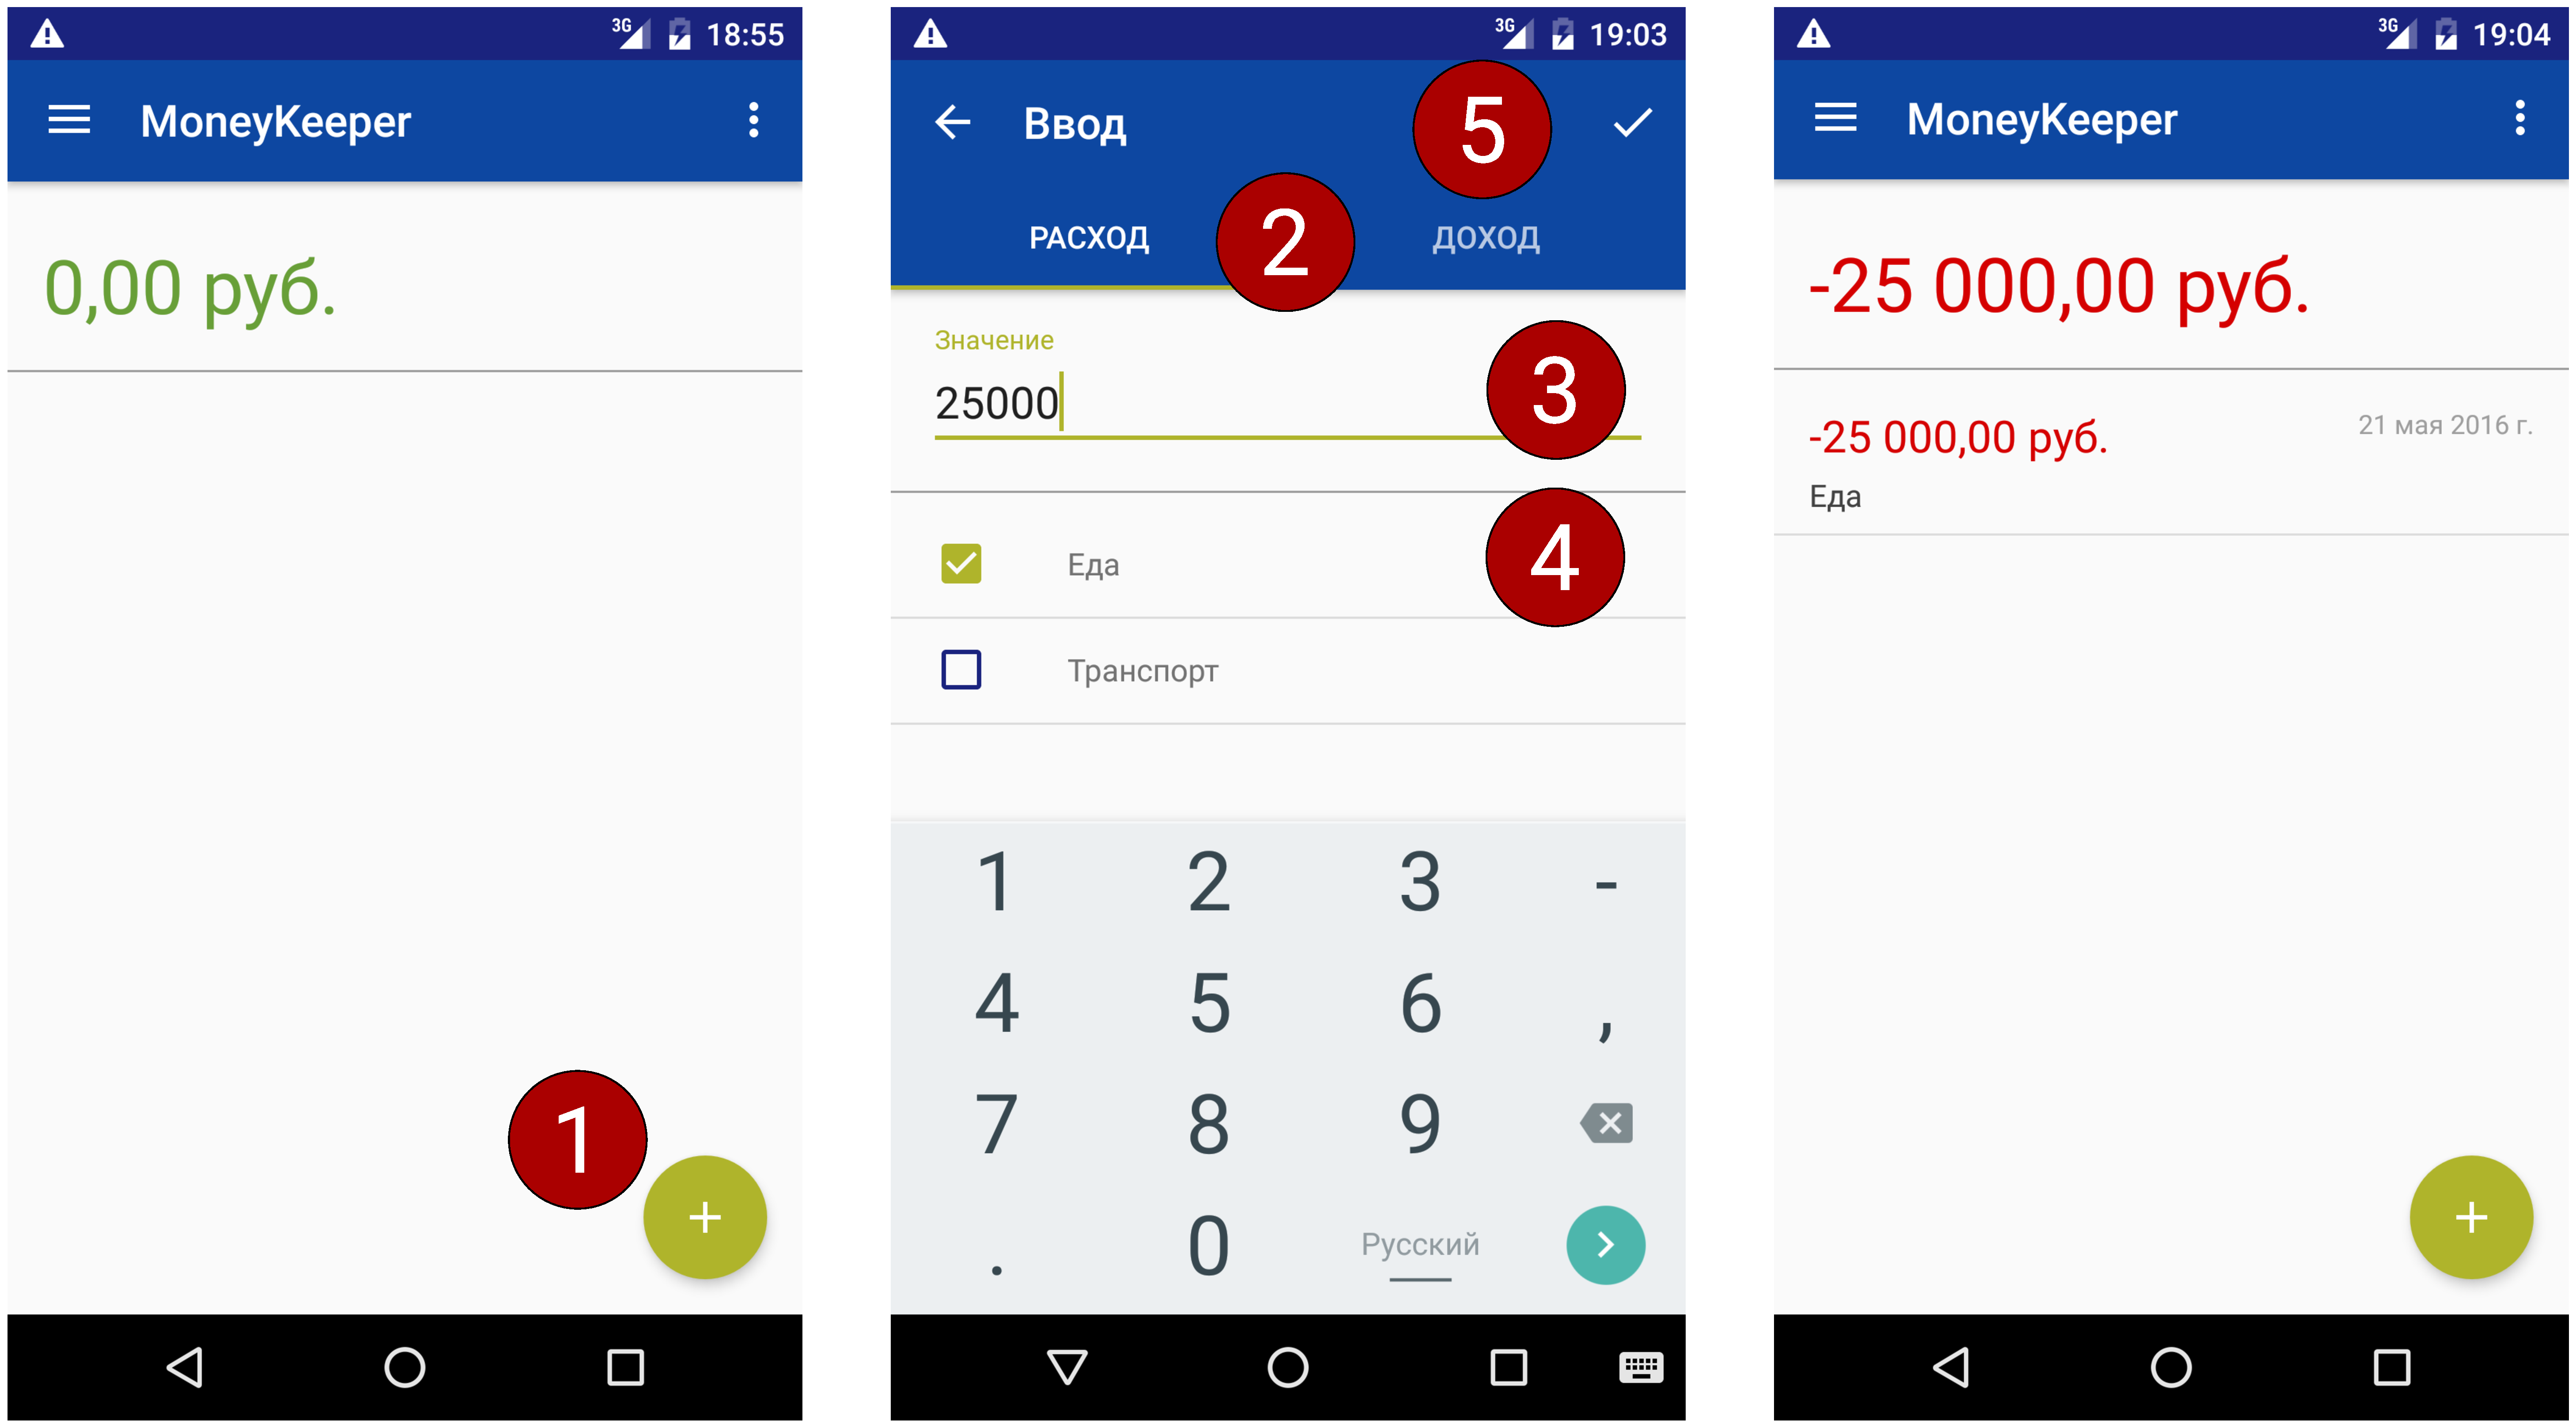
\includegraphics[width=\textwidth]{fig/implementation_manual_balance_change.eps}
\end{frame}

\begin{frame}{Технико-экономическое обоснование}
  Приложение открытое и бесплатное.

  Затраты: \( \approx 184 \) ч., \( \approx 46 \) млн. б. р.

  \smallskip
  Социальный эффект:
  \begin{itemize}
  \item сокращение времени на учет;
  \item анализ затрат \( \Rightarrow \) сокращение затрат.
  \end{itemize}
\end{frame}

\begin{frame}{Перспективы развития}
  \begin{itemize}
  \item повышение точности распознавания числовых данных;
  \item учет переводов денежных средств;
  \item сортировка категорий учета на основании \\
    данных о местоположении.
  \end{itemize}
\end{frame}

\begin{frame}{Выводы}
  \begin{itemize}
  \item ???
  \item исходный код: \url{https://github.com/budnyjj/MoneyKeeper.git}.
  \end{itemize}
\end{frame}

\begin{frame}{Конец}
  \centering
  Спасибо за внимание!
\end{frame}

\end{document}